\section{Fixed-D10 temporal confirmation}\label{sec:c5}
\subsection{Frozen roles and complete execution}
A separately authorized temporal confirmation assessed D11, D12 and D13 using R1--R6 and R8--R13. The twelve frozen RF models were fitted only on D1, D2 and D4--D9, with the same seed 487, 100 trees, depth 5, minimum leaf size 5 and fit-only scaling. Initial correction calibration and scheduler normalization used D10 only. Every policy, budget, seed and assessment session reset independently to that same D10 state; no rolling recalibration or final-label carry occurred. R7/R14 and the UCI270 reservations remained excluded.

The complete predeclared comparison retained the two original primary contrasts, all five schedules, budgets 0/5/10/20, all random seeds 487--496, and the declared forgetting and fixed $.95$ information-controller extensions. Each current prediction, raw/reported interval and decision was persisted before purchase; a purchased reference affected later predictions only. All 129 replay paths and 12,900 pre-query records were committed before final performance summaries. A saved-output arithmetic audit reproduced all 40,635 per-run metric rows exactly, verified the fixed initial states and causal records, and checked unchanged source/model/development hashes. No integrity/access violation or numerical-update failure was found. The 300 exposures and 3,600 correlated outputs are separate from the development sample.

\subsection{Frozen benefit criterion and primary findings}
The criterion fixed before confirmation requires lower strict 1 ppm exceedance and nonpositive MAE change pooled and in both families. It applies separately to historical affine B0 versus unchanged consensus and to affine envelope B20 versus its own B0. Uniform-session improvement additionally requires no adverse session/family cell. The secondary schedule-superiority rule requires favorable exceedance and nonpositive MAE against periodic, random-seed mean and confidence, pooled and in both families (Section~\ref{sec:evaluation}).
Table~\ref{tab:c5primary} retains the pooled and both-family results. Historical affine correction reduces pooled MAE from 1.4570 to 1.3553 ppm and strict 1 ppm exceedance from 1,791/3,600 to 1,550/3,600 (49.75\% to 43.06\%). Figaro contributes 240 of the 241 net removed exceedances. FIS MAE instead increases from 0.8820 to 0.9471 ppm, worsening on all three sessions. Thus the frozen historical-benefit criterion requiring favorable exceedance and nonpositive MAE change in both families is not met; the finding is heterogeneous.

\begin{table}[H]\centering\small
\caption{Fixed-D10 temporal confirmation, distinct from development. MAE in ppm; counts are strict 1 ppm exceedances. B0 and envelope B20 use cumulative inverse affine correction. $N$ counts correlated configuration outputs, not independent exposures.}\label{tab:c5primary}
\setlength{\tabcolsep}{4pt}\begin{tabular}{lrrrrrrr}
\toprule
Scope & $N$ & Raw MAE & B0 MAE & B20 MAE & Raw count & B0 count & B20 count \\ \midrule
ALL & 3600 & 1.4570 & 1.3553 & 1.3257 & 1791 & 1550 & 1517 \\
Figaro & 1800 & 2.0320 & 1.7636 & 1.7481 & 1275 & 1035 & 1019 \\
FIS & 1800 & 0.8820 & 0.9471 & 0.9033 & 516 & 515 & 498 \\
\bottomrule\end{tabular}\end{table}


The original incremental comparison, cumulative affine envelope B20 against its own B0, reduces pooled MAE by 0.0297 ppm to 1.3257 ppm and exceedance by 33 outputs to 1,517/3,600 (42.14\%). Both family-aggregate MAE and exceedance changes are favorable, satisfying the prespecified descriptive incremental-benefit criterion. FIS improves relative to affine B0 (0.9471 to 0.9033 ppm), but its MAE remains worse than unchanged consensus (0.8820 ppm). This does not establish uniform improvement: pooled D12 MAE changes by +0.0049 ppm; Figaro/FIS D12 changes are +0.0071/+0.0027 ppm, and FIS D13 changes by +0.0068 ppm with one additional exceedance. Pooled D11/D13 MAE changes are $-0.0918/-0.0021$ ppm. All session/family numerators and denominators are in Supplement S10 and the full numerical files.

\begin{figure}[H]\centering
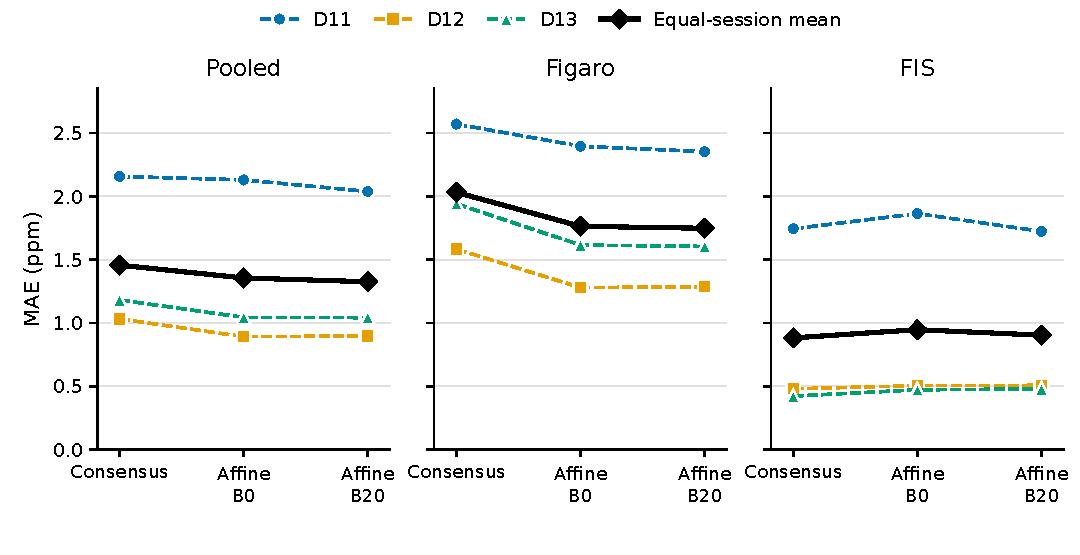
\includegraphics[width=\linewidth]{fig_4_c5_primary_mae.pdf}
\caption{Prespecified primary confirmation paths, with a shared vertical scale. D11 circles, D12 squares and D13 triangles show session MAE; black diamonds show equal-session means. Lines connect unchanged consensus, cumulative affine B0 and cumulative affine envelope B20, using the same frozen RF models and independent D10 resets. Each pooled session has 1,200 outputs and each family has 600 from 100 shared exposures. FIS B20 remains worse than consensus in aggregate; all session reversals remain visible.}\label{fig:c5mae}
\end{figure}

Fourteen of the fifteen pooled affine B20 MAE point changes are favorable in confirmation, whereas all fifteen were adverse in development. The confidence $.90$ change is adverse (+0.0047 ppm); confidence $\lambda=1$ improves MAE while worsening strict exceedance. The native $.95$ comparator changes pooled MAE by $-0.0551$ ppm, but remains an extension rather than a replacement primary. No method, factor, budget, family or seed was selected by its final outcome. Secondary envelope-schedule superiority is not established: against confidence at $\lambda=1$ B20, envelope has worse pooled MAE (+0.0078 ppm) and worse FIS MAE and exceedance.

\subsection{Scientific bound failures in a valid evaluation}
Table~\ref{tab:c5intervals} separates raw noncontainment, reported-set noncontainment, contradictions and actual midpoint false assurance. Envelope B20 has 284/3,600 raw noncontainments and 276/3,600 reported noncontainments, with eight contradictory outputs contained only by the descriptive hull. Mean width is 15.7129 ppm. Of 74 midpoint flags at 1 ppm, 38 are false: 38/74=51.35\% conditional and 38/3,600=1.06\% overall. Figaro contributes 1/1 false/assured and FIS 37/73. Queried outputs have 8/14 false/assured and 8/720 false/all; unqueried outputs have 30/60 and 30/2,880. These are midpoint-envelope diagnostics, not affine uncertainty intervals; RLS assurance remains unavailable.

\begin{table}[H]\centering\small
\caption{Primary envelope B20 interval diagnostics in confirmation. Outside counts use raw intersection and reported set separately. False/assured refers to actual midpoint error above 1 ppm among noncontradictory own-radius flags.}\label{tab:c5intervals}
\setlength{\tabcolsep}{4pt}\begin{tabular}{lrrrrrr}
\toprule
Scope & $N$ & Raw out & Report out & Contradictions & Width (ppm) & False/assured \\ \midrule
ALL & 3600 & 284 & 276 & 8 & 15.7129 & 38/74 \\
Figaro & 1800 & 56 & 56 & 0 & 25.4683 & 1/1 \\
FIS & 1800 & 228 & 220 & 8 & 5.9575 & 37/73 \\
\bottomrule\end{tabular}\end{table}


These failures reject an unconditional hard-bound claim and remain scored scientific outcomes. They do not invalidate the otherwise verified evaluation. No confirmation bootstrap, bound retuning, model refit, favorable-seed selection or experiment repeat was performed. This is later-session evidence on the same apparatus, not certified physical uncertainty, independent-array validation or a new algorithmic claim.
